% Vorlage: https://www.pfsr.de/latex

% -- Anfang Präambel
\documentclass[german,  % Standardmäßig deutsche Eigenarten, englisch -> english
parskip=full,  % Absätze durch Leerzeile trennen
%bibliography=totoc,  % Literatur im Inhaltsverzeichnis (ist unüblich)
%draft,  % TODO: Entwurfsmodus -> entfernen für endgültige Version
]{scrartcl}

\usepackage[utf8]{inputenc}  % Kodierung der Datei
\usepackage[T1]{fontenc}  % Vollen Umfang der Schriftzeichen
\usepackage[ngerman]{babel}  % Sprache auf Deutsch (neue Rechtschreibung)

% Mathematik und Größen
\usepackage{amsmath}
\usepackage[locale=DE,  % deutsche Eigenarten, englisch -> US
separate-uncertainty,  % Unsicherheiten seperat angeben (mit ±)
]{siunitx}
\usepackage{physics}  % Erstellung von Gleichungen vereinfachen

\usepackage{graphicx}  % Bilder einbinden \includegraphics{Pfad/zur/Datei(ohne Dateiendung)}

% Gestaltung
\usepackage{booktabs}  % schönere Tabellen
\usepackage[toc]{multitoc}  % mehrspaltiges Inhaltsverzeichnis
\usepackage{csquotes}  % Anführungszeichen mit \enquote
\usepackage{caption}  % Anpassung der Bildunterschriften, Tabellenüberschriften
\usepackage{subcaption}  % Unterabbildungen, Untertabellen, …
\usepackage{enumitem}  % Listen anpassen
\setlist{itemsep=-10pt}  % Abstände zwischen Listenpunkten verringern

% Manipulation des Seitenstils
\usepackage[headtopline = .5pt]{scrlayer-scrpage}

% Bibliographie
\usepackage[backend=biber]{biblatex}
\addbibresource{bibliography.bib}

% SI-Einheiten darstellen
\usepackage{siunitx}

% Code - Blöcke
\usepackage{listings}
\usepackage[dvipsnames]{xcolor}

% Kopf-/Fußzeilen setzen
\pagestyle{scrheadings}  % Stil für die Seite setzen
\clearmainofpairofpagestyles  % Stil zurücksetzen, um ihn neu zu definieren
\automark{section}  % Abschnittsnamen als Seitenbeschriftung verwenden
\ofoot{\pagemark}  % Seitenzahl außen in Fußzeile
\ihead{\headmark}  % Seitenbeschriftung mittig in Kopfzeile

\usepackage[hidelinks]{hyperref}  % Links und weitere PDF-Features

% TODO: Titel und Autor, … festlegen
\newcommand*{\titel}{Elektronische Detektorauslese und digitale Datenverarbeitung mit FPGA}
\newcommand*{\autor}{Sebastian Thiede, Alexander Lettau}
\newcommand*{\abk}{FP}
\newcommand*{\betreuer}{Johann C. Voigt}
\newcommand*{\messung}{22.11.2021 \& 24.11.2021}
\newcommand*{\ort}{ASB/K07}

\hypersetup{pdfauthor={\autor}, pdftitle={\titel}}  % PDF-Metadaten setzen

% automatischen Titel konfigurieren
\titlehead{Praktikum des IKTP \abk \hfill TU Dresden}
\subject{Versuchsprotokoll}
\title{\titel}
\author{\autor}
\date{\begin{tabular}{ll}
Protokoll: & \today\\
Datum Praktikum: & \messung\\
Ort: & \ort\\
Betreuer: & \betreuer\end{tabular}}

\lstset{ % General setup for the package
    language=VHDL,
    basicstyle=\small\sffamily,
    numbers=left,
    numberstyle=\tiny,
    frame=single,
    tabsize=4,
    columns=fixed,
    showstringspaces=false,
    showtabs=false,
    keepspaces,
    breaklines=true
    commentstyle=\color{OliveGreen},
    keywordstyle=\color{blue},
    identifierstyle=\color{black}
}

\renewcommand\lstlistingname{Quelltext} % Change language of section name

% -- Ende Präambel

\begin{document}
\begin{titlepage}
\maketitle  % Titel setzen
\tableofcontents  % Inhaltsverzeichnis setzen
\end{titlepage}

% ----- DOKUMENT ANFANG -----

\section{Workshop}
In dem Workshop haben wir gelernt wie man VHDL schreibt, wie man VHDL-Dateien simuliert und synthetisiert und wie man synthetisierte Dateien auf einen Hardware FPGA überträgt.
Zu beachten ist dabei, dass wir selbst immer nur einen Teil der VHDL-Dateien ergänzt haben um im Praktikum Zeit zu sparen.
Es sei nochmal darauf hingewiesen dass ein FPGA von sich aus nicht sequentiell arbeitet.
Einige Formulierungen von Verarbeitungsabläufen könnten als zeitliche Abfolge fehlinterpretiert werden.
Dies ist jedoch nur der Fall wenn dies explizit erwähnt wird.

\subsection{Beispiel - NAND-Gatter}
Das erste Beispiel das wir uns angeschaut haben ist ein NAND-Gatter.
Anhand von diesem wollen wir die grundlegende Syntax erklären.
Dazu ist hier der verwendete Code:

\lstinputlisting[firstline = 10]{../Daten/example/example.vhd}

Die ersten beiden Zeilen binden aus der Bibliothek \textbf{IEEE} den Datentyp \textbf{std\_logic} ein, der im Wesentlichen einen boolean darstellt.
Daraufhin wird in Zeile $4$ eine \textbf{entity} erstellt.
Diese stellen Schnittstellen für Logikbausteine dar.
Im Abschitt \textbf{port} werden Verbindungen nach außen definiert.
Es wird mittels der Schlüsselwörter \textbf{in} und \textbf{out} definiert welche Signale als Ein- und Ausgänge genutzt werden, und es wird ihnen ein Typ zugewiesen.
Außerdem können diese Signale initialisiert werden wie z.B. in Zeile $8$.
Später werden wir auch den Abschnitt \textbf{generic} verwenden, mit dem die \textbf{entity} parametrisiert werden kann um einfache Variationen von Instanzen zu ermöglichen.
Das erstellen der \textbf{entity} wird in Zeile $10$ beendet.

In Zeile $12$ wird eine \textbf{architecture} erstellt die die Funktionalität der eben erstellten \textbf{entity} beschreibt.
Darauf wird ein internes \textbf{std\_logic} Signal, auf das von außen nicht zugegriffen werden kann, erstellt und initialisiert.
Im Folgenden wird die eigentliche Logik des NAND-Gatters implementiert.
Dazu wird dem internen Signal das Ergebnis der boolschen AND Verknüpfung zugewiesen und dem Ausgabesignal der negierte Wahrheitswert des internen Signals.
Hierbei ist zu beachten dass diese Zuweisung nicht sequenziell passiert, sondern das tatsächliche Verknüpfungen der Signale durch Gatter gemeint sind.
Eine Änderung des Eingangssignals wirkt sich damit (bis auf Signallaufzeiten) sofort auf den Ausgang aus.
Es ist daher auch nicht wichtig in welcher Reihenfolge diese Verknüpfungen aufgelistet sind.
In Zeile $19$ wird dann schlussendlich das Beschreiben der \textbf{architecture} beendet.

\subsection{Übung - Logische Gatter}

In der ersten Übung sollten drei LEDs mithilfe von drei Schaltern und einem Knopf nach bestimmten Bedingungen angesteuert werden. Diese lauten:
\begin{itemize}
    \item Sind alle Schalter an soll LED $0$ an sein (sonst aus)
    \item Sind mindestens zwei der Schalter an soll LED $1$ an sein (sonst aus)
    \item Ist Schalter $2$ an und der Knopf nicht gedrückt soll LED $2$ an sein (sonst aus)
\end{itemize}

Dazu haben wir folgende VHDL Datei erstellt:

\lstinputlisting[firstline = 10]{../Daten/gates/gates.vhd}

In der Beschreibung der \textbf{entity} \textbf{gates} sind die drei Schalter und der Knopf als Eingang, sowie die drei LEDs als Ausgang zu erkennen.
Um die Funktionalität zu implementieren wurde in der \textbf{architecture} jedem LED-Ausgangssignal eine entsprechende Logikverknüpfung der Eingangssignale zugewiesen.
So wurde zum Beispiel für die LED $1$ die Signale der Schalter jeweils Paarweise AND verknüpft und die Ergebnisse davon OR verknüpft.

\begin{figure}[ht]
	\centering
    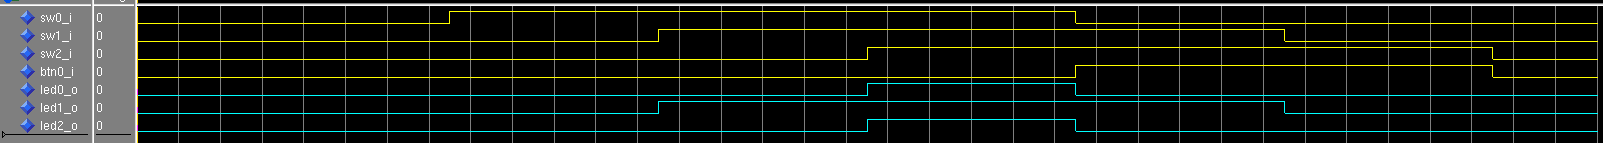
\includegraphics[width=0.98\textwidth]{../Daten/gates.png}
	\caption{Simulation von gates.vhd}
	\label{img_gates}
\end{figure}

In Abb. \ref{img_gates} wurde diese VHDL Datei simuliert.
Man sieht dass die gewünschte Funktionalität gegeben ist:
\begin{itemize}
    \item LED $0$ ist nur an wenn alle Schalter an sind
    \item LED $1$ ist an solange mindestens zwei Schalter an sind
    \item LED $2$ ist an wenn Schalter $2$ an und der Knopf nicht gedrückt ist
\end{itemize}

Wir haben diese VHDL-Datei außerdem synthetisiert und dem FPGA aufgespielt um die Funktionalität zu überprüfen.
Es funktionierte einwandfrei.
Ein Bild von einer beispielhaften Schalterstellung ist in Abb. \ref{photo_gates} zu sehen.

\begin{figure}[ht]
	\centering
    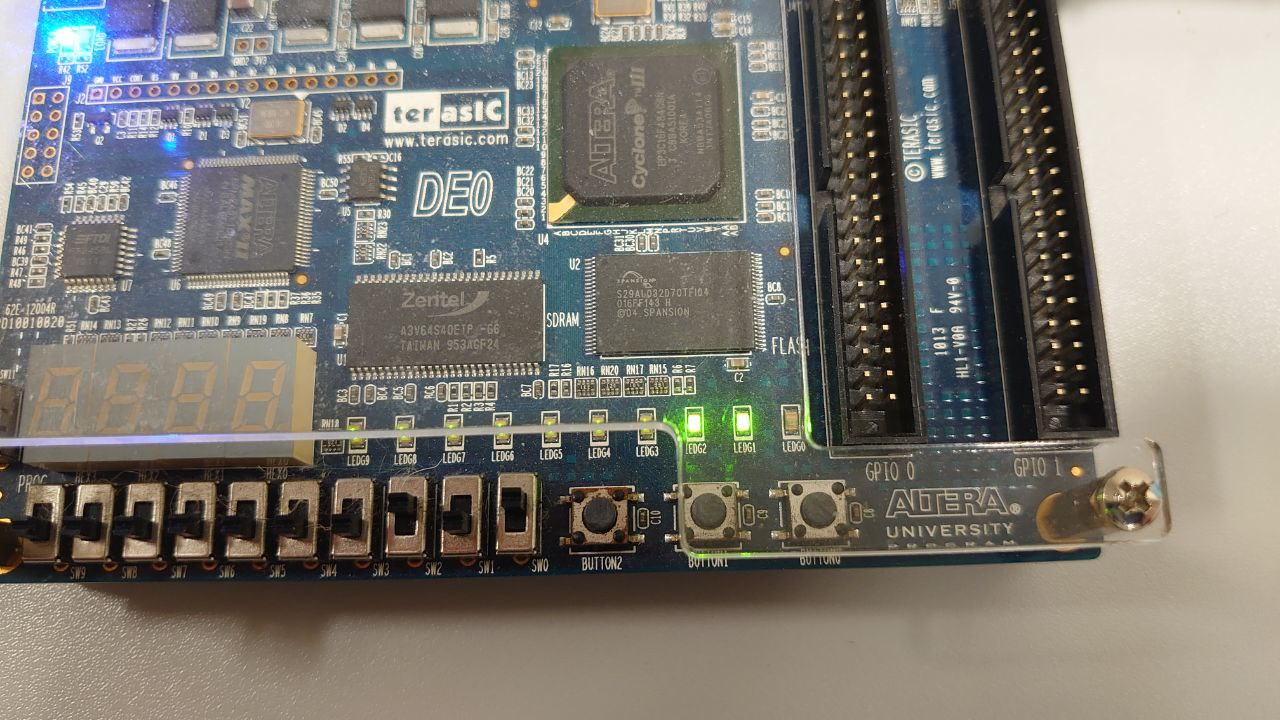
\includegraphics[width=0.98\textwidth]{../Daten/Photo_FPGA_gates.png}
	\caption{Photo des FPGA mit aufgespielter, synthetisierter Verknüpfung von gates.vhd in beispielhafter Schalterstellung. Da nur Schalter $0$ und $2$ an (und der Knopf nicht gedrückt) sind sollten LED $1$ und $2$ an sein, und sie sind es.}
	\label{photo_gates}
\end{figure}

\subsection{Modul 1 - \textit{LoHi detect}}

Ab hier wurde an dem Projekt für die Datenverarbeitung am ATLAS Kalorimeter gearbeitet.
In solchen Anwendungen wird üblicherweise mit einer \textit{Clock}, einem Taktsignal gearbeitet.
Die Clock ermöglicht es der Datenverarbeitung nun auch eine Zeitdimension (neben Signallaufzeiten im FPGA) zu geben.
Da wir hier mit vorgefertigten Daten arbeiten müssen wir ein Startsignal zum Senden der Daten von außerhalb (vom PC) geben.
Dafür verwenden wir einen Knopf.
Um das Senden der Daten nur einmal und in definierter Weise auszulösen müssen wir den Knopfdruck an die Clock koppeln.
Dafür ist das Modul \textit{LoHi detect} zuständig.
Die Aufgabe bestand darin das ausgehende Signal (sig\_o) dann auf $1$ zu setzen wenn zu einer steigenden Flanke der Clock der Knopf gedrückt ist, zur wiederum nächsten steigenden Flanke der Clock sollte es jedoch wieder auf $0$ gesetzt werden.
Im Folgenden ist der Code dieses Moduls zu sehen:

\lstinputlisting[firstline = 10]{../Daten/lohi_detect/lohi_detect.vhd}

Hier wurde ein neues Syntaxelement genutzt: der \textbf{process}.
Dieser tritt innerhalb der \textbf{architecture} auf und wird immer dann ausgeführt wenn eines der Signale die nach dem Schlüsselwort \textbf{process} aufgezählt werden sich ändert.
Im Gegensatz zum Großteil der restlichen VHDL Syntax wird innerhalb eines \textbf{process} sequentiell gearbeitet.
Eine Änderung der Signale findet jedoch erst statt wenn der Prozess beendet ist.
Dadurch sind \textbf{if} Bedingungen und Schleifen möglich.
Intern (beim synthetisieren) werden diese jedoch aufgedröselt, denn im FPGA läuft nichts tatsächlich sequentiell ab.
In dem Code-Beispiel wird also zu jeder steigenden Flanke der Clock dem Ausgangssignal der Wert des Knopfes AND verknüpft mit dem inversen des internen Signal reg zugewiesen.
Dies ist zum ersten Clock-Zyklus eine $1$.
Dem interne Signal reg wiederum wird der Wert des Eingangssignals zugewiesen.
Das verhindert das im nächsten Clock-Zyklus das Eingangssignal auf das Ausgangssignal übergeht; Stattdessen wird das Ausgangssignal $0$.
Solange der Knopf gedrückt bleibt ändert sich daran nichts.
Wird der Knopf losgelassen wird zur nächsten steigenden Flanke der Clock das interne Signal auf $0$ gesetzt und man befindet sich im Ausgangszustand.

\begin{figure}[ht]
	\centering
    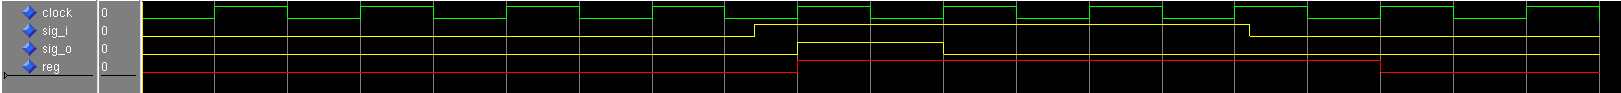
\includegraphics[width=0.98\textwidth]{../Daten/lohi_detect.png}
	\caption{Simulation von lohi\_detect.vhd}
	\label{img_lohi_detect}
\end{figure}

In Abb. \ref{img_lohi_detect} wurde dieses Modul simuliert.
Man sieht das nach Betätigung des Knopfes zur nächsten steigenden Flanke der Clock der Ausgang einen Zyklus lang auf $1$ steht.
Als der Knopf losgelassen wird und das Eingangssignal wieder auf $0$ fällt wird zur nächsten steigenden Flanke der Clock auch das interne Signal reg zurückgesetzt.

\subsection{Modul 2 - \textit{Max find}}

Die Aufgabe des Moduls \textit{Max find} ist es das Maximum einer Folge von Daten zu bestimmen.
Die Konvention ist, dass zu jeder steigenden Flanke der Clock ein neuer Eingangswert (nächstes Folgenglied) vorliegt.
VHDL hat eine Implementierung verschiedener Datentypen die wir hier verwenden.
Diese sind in der Bibliothek IEEE.numeric\_std zu finden die jetzt mit eingebunden wird:

\lstinputlisting[firstline = 10]{../Daten/max_find/max_find.vhd}

Auch hier arbeiten wir wieder mit den Daten, die von außen eingespeist werden (vom PC), und brauchen daher ein Startsignal.
Es heißt hier start\_i.
Wie in der entity max\_find schon zu sehen ist, verwenden wir für die eingehenden und ausgehenden Daten den Typ \glqq signed\grqq{}, der eine ganze Zahl (mit Vorzeichen) darstellt.
Die Bitweite bestimmt hierbei den Wertebereich. Dieser bestimmt sich bei signed zu $[-2^{bit\_width - 1}, 2^{bit\_width - 1} - 1]$.
In unserem Fall (Bitweite $14$) also $[-8192, 8191]$.
\glqq integer \grqq{} ist sehr ähnlich zu signed, nur das dort weitere arithmetische Operationen definiert sind.
Ein \glqq unsigned \grqq{} hat den Wertebereich $[0, 2^{bit\_width} - 1]$ (auch ganzzahlig).
Man kann zwischen all diesen Typen mit entsprechenden Befehlen konvertieren.

Die \textbf{architecture} von max\_find verwendet ein internes Signal \glqq reg\grqq{} welches immer das Ausgangssignal liefert (Zeile $33$).
Das interne Signal kann innerhalb vom \textbf{process} geändert werden, das Ausgangssignal jedoch nicht.
Zu jeder steigenden Flanke der Clock wird reg auf $0$ gesetzt wenn das Startsignal gegeben wird.
Ist dies nicht der Fall wird überprüft ob das Eingangssignal einen größeren Zahlenwert hat als das Signal reg.
Ist dies der Fall wird reg auf den Wert des Eingangssignals gesetzt, ansonsten passiert nichts.
Damit wird nach Erhalten des Startsignals immer nur der größte Zahlenwert beibehalten.

\begin{figure}[ht]
	\centering
    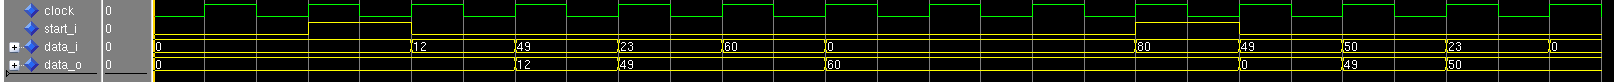
\includegraphics[width=0.98\textwidth]{../Daten/max_find.png}
	\caption{Simulation von max\_find.vhd}
	\label{img_max_find}
\end{figure}

Das Verhalten des Moduls wurde in Abb. \ref{img_max_find} simuliert.
Folgende Dinge sind zu beobachten:
Nach dem Auftreten des Startsignals werden Eingangswerte aufgezeichnet.
Es dauert einen Takt zusätzlich bis das Maximum aktualisiert wird.
Tritt ein kleinerer Wert auf als das bisherige Maximum wird dieser natürlich nicht übernommen.
Ein weiteres Startsignal setzt das Maximum auf $0$ zurück.
Eingangswerte während des Startsignals werden nicht aufgezeichnet.
Insgesamt verhält sich das Modul wie gewünscht.

\subsection{Modul 3 - \textit{filter}}

Das Modul \textit{filter} wendet einen Wiener Filter auf die Eingangswerte an.
Es handelt sich dabei um eine gewichtete Summe der letzten sechs Eingangswerte.
Dies wird bei der Datenauswertung verwendet um Rauschen zu unterdrücken.
Im Folgenden ist der Code dieses Moduls zu sehen:

\lstinputlisting[firstline = 11]{../Daten/filter/filter.vhd}

Die Wichtungskonstanten sind in den Zeilen $29$ bis $34$ zu finden.
Sie werden in einem \textbf{array} des Typs integer gespeichert.
Da das Rechnen mit (Fest-)Kommazahlen einige Schwierigkeiten mit sich bringt werden die Konstanten mit einem gemeinsamen Faktor $2^{k}$ multipliziert.
Dieser Faktor wird hinterher wieder herausdividiert, indem die unteren $k$ Bit des Ergebnisses abgeschnitten werden (entspricht in Binär einer Division durch $2^{k}$).
Man kann also die Ausgabe des Filters schreiben als
\begin{gather}
    y_{n} = \frac{\sum_{i=0}^{5} (2^{k} \cdot c_{i+1}) \ x_{n-i}}{2^{k}}
    \label{equation_module_filter}
\end{gather}
wobei $(2^{k} \cdot c_{i+1})$ die im Modul gelisteten Konstanten $c(1)$ bis $c(6)$ mit $k = \text{shif} = 15$ sind.
Die $x_{n-i}$ sind die letzten Eingangswerte und für $i=0$ der aktuelle Eingangswert.
In der \textbf{architecture} der \textbf{entity} des Moduls \textit{filter} werden zwei interne Signale verwendet: data\_uns (Zeile $37$) und buf (Zeile $40$).
data\_uns ist der Zähler in Gleichung \ref{equation_module_filter}.
In Zeile $66$ ist zu sehen, dass das Ausgangssignal wie erwähnt auf die oberen Bits bis zu shif aus data\_uns gekürzt wird.
buf wird verwendet um die letzten fünf Eingangssignale zu speichern.
Um schließlich die Berechnung durchzuführen wird wieder ein \textbf{process} verwendet der zur steigenden Flanke der Clock ausgeführt wird.
Diesmal verwenden wir außerdem eine \textbf{variable} par\_sum um iterativ den Zähler in Gleichung \ref{equation_module_filter} zu bestimmen.
In den Zeilen $48$ bis $51$ werden die Werte aktualisiert (weitergeschoben, der neue Eingangswert wird in buf(0) gespeichert).
Man muss an dieser Stelle daran erinnern, dass die Änderungen der Werte in buf erst zum Ende des \textbf{process} wirksam werden.
In Zeile $53$ wird nun par\_sum mit dem ersten Term initialisiert.
In der darauffolgenden for-Schleife werden die übrigen Terme mit den alten Werten in buf aufsummiert.
Zum Schluss wird das interne Signal data\_uns auf das Ergebnis der Summation gesetzt, mit Typenkonversion von integer zu signed.
Damit sollte am Ausgang Gleichung \ref{equation_module_filter} realisiert sein.

\begin{figure}[ht]
	\centering
    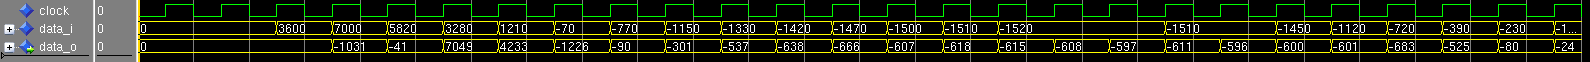
\includegraphics[width=0.98\textwidth]{../Daten/filter.png}
	\caption{Simulation von filter.vhd}
	\label{img_filter}
\end{figure}

Dies wird wieder mit einer Simulation überprüft; sie ist in Abb. \ref{img_filter} zu sehen.
Man sieht das das Ausgangssignal einen Takt nach dem Auftreten des ersten Eingangswerts von $0$ verschieden ist.
Auch sieht man das der erste Wert negativ ist, da $c(1)$ negativ ist.
Der Leser sei versichert, dass die Ausgabewerte zahlenmäßig den Erwartungen entsprechen.
Tritt in zwei aufeinanderfolgenden Takten dasselbe Eingangssignal auf werden diese natürlich trotzdem als neue Werte gesehen und das Ausgangssignal passt sich im nächsten Zyklus an.
Auch hier läuft also alles wie gewünscht.

\subsection{Übung - Sekundenzähler}

Da wir an unserem FPGA sehen wollen was gerade passiert ist es notwendig die eingebauten 7-Segment-Anzeigen anzusteuern.
Dafür wurde freundlicherweise bereits ein Modul bereitgestellt welches die Zuordnung der Zahlen $0$ bis $9$ zu den entsprechenden LEDs der 7-Segment-Anzeigen übernimmt.
Um sich mit dem Umgang mit diesem Modul vertraut zu machen wurde ein einfacher Sekundenzähler implementiert.
Dieser soll von $0$ bis $9$ Sekunden zählen und sich dann auf $0$ zurücksetzen.
Im Folgenden ist der Code des Sekundenzählers zu sehen:

\lstinputlisting[firstline = 12]{../Daten/ssd/seconds.vhd}

Die \textbf{entity} seconds besitzt zwei \textbf{generic}s: counter\_max und invert.
counter\_max ist der Wert bis zu welchem später gezählt wird bis eine Sekunde vergangen ist.
Dies ist notwendig da die Clock eine sehr viel höhere Taktfrequenz als \SI{1}{\hertz} hat.
invert wird verwendet um die Bits des Ausgangs zu invertieren, also Segmente der 7-Segment-Anzeige zu invertieren.
Dies kann notwendig sein da 7-Segment-Anzeigen je nach Bauart mit gemeinsamer Kathode ($1$ = Segment an) oder gemeinsamer Anode ($0$ = Segment an) vorkommen.
Da invert auf wahr gesetzt wird lässt sich folgern das im FPGA 7-Segment-Anzeigen mit gemeinsamer Anode verbaut sind.
Der Ausgang ist in Zeile $12$ definiert.
Es handelt sich um einen \textbf{std\_logic\_vector}, ein \textbf{array} von \textbf{std\_logic}, mit einem Eintrag für jedes Segment.
Er wird auf $0$ initialisiert (alle Segmente aus).

Die \textbf{architecture} hat drei interne Signale: sec, counter und B.
sec gibt einfach an welche Zahl auf dem Display stehen soll.
counter wird wie erwähnt verwendet um bis zur vollen Sekunde zu zählen.
B ist ein Hilfssignal, dass eine binäre Repräsentation von sec hält.
Wieder wird ein \textbf{process} bei steigender Flanke der Clock ausgeführt.
In jedem Fall wird der counter um eins erhöht.
Ist der counter eins vor counter\_max ist eine Sekunde vergangen.
Dies wird mithilfe einer \textbf{if} Bedingung überprüft.
Dann wird überprüft ob die Anzeige bisher bei $9$ Sekunden stand.
Ist dies der Fall wird alles auf $0$ gesetzt (Zeilen $32$ bis $34$).
Ansonsten werden die gezählten Sekunden um eins erhöht und der counter auf $0$ gesetzt (Zeilen $36$ bis $38$).

Das mapping der Sekunden zu den Segmenten der Anzeige wird wie gesagt über das Modul \textit{single\_disp} abgewickelt.
Dazu wird in Zeile $45$ eine \textbf{entity} dieses Moduls erstellt.
In den folgenden Zeilen wird dann angegeben welches Signal im Modul \textit{single\_disp} mit welchem Signal aus dem Sekundenzähler korrespondiert.
Es handelt sich dabei wieder um feste, quasi-instantane Verbindungen.

\begin{figure}[ht]
	\centering
    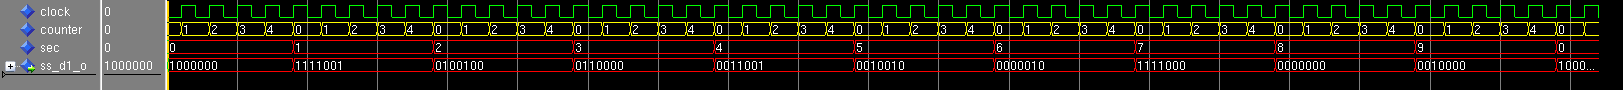
\includegraphics[width=0.98\textwidth]{../Daten/seconds2.png}
	\caption{Simulation von seconds.vhd}
	\label{img_seconds}
\end{figure}

Dieses Modul wurde ebenfalls simuliert, zu sehen in Abb. \ref{img_seconds}.
Um nicht bis zu riesigen Zahlen zu zählen wurde in der Simulation counter\_max auf $5$ gesetzt.
Es ist schnell zu erkennen das nach immer $5$ steigenden Flanken der Clock eine Sekunde dazugezählt wird.
Ganz rechts ist auch das Zurücksetzten auf $0$ zu erkennen.
Man macht sich auch ohne Kenntnis der genauen Belegung der Segmente durch zählen der Nullen in der letzten Zeile klar, dass tatsächlich die richtige Zahl angezeigt wird.
Dies ist genau das gewünschte Verhalten.

Dies wurde auch durch synthetisieren und aufspielen des Moduls auf den FPGA überprüft.
Leider haben wir dafür kein Bild, es sei aber versichert, dass alles wie gewünscht geklappt hat.

\subsection{Modul 4 - \textit{ssd}}
Die Werte die Dargestellt werden sollen sind vierstellig.
Daher ist es notwendig die Stellen zu trennen und einzeln darzustellen.
Das ist die Aufgabe des Moduls \textit{ssd} (seven-segment-display). Der Code dieses Moduls ist im Folgenden gegeben:

\lstinputlisting[firstline = 12]{../Daten/ssd/ssd.vhd}

Die vier Ausgangssignale sind ss\_d1\_o bis ss\_d4\_o welche jeweils die LEDs der 7-Segment-Anzeigen repräsentieren.
Um die Funktionalität dieses Moduls zu implementieren wurde in der \textbf{architecture} der Befehl \textbf{generate} verwendet.
Dieser ermöglicht es einen Code-Baustein leicht abgewandelt zu duplizieren (wird vom Compiler durchgeführt).
Er wird hier verwendet um alle 7-Segment-Anzeigen auf einmal zu behandeln.
Zuerst werden die Dezimalstellen in Zeile $45$ voneinander getrennt und im internen Signal quotient gespeichert.
Wir nehmen zum besseren Verständnis die Zahl $1234$ als Beispiel und wollen uns ansehen wie die zweite Dezimalstelle von links, also die $2$, herausgetrennt wird.
Dafür wird das Eingangssignal in einen integer umgewandelt, da für diesen Datentyp die algebraischen Operationen Division und Modulo implementiert sind.
Dann wird durch eine Zehnerpotenz geteilt, sodass die Dezimalstelle von Interesse gerade die Stelle links vom Komma ist.
Der nicht-ganzzahlige Anteil wird dabei automatisch abgeschnitten.
Für unser Beispiel wird also durch $100$ geteilt und es bleibt $12$.
Weiterhin werden größere Dezimalstellen abgetrennt durch das Modulo $10$.
In unserem Beispiel bleibt damit $2$ übrig und wir haben die richtige Dezimalstelle isoliert.
Zuletzt wird wieder in einen signed mit $5$ bit umgewandelt um über das Modul \textit{single\_disp} die entsprechenden LED-Ansteuerungen herauszusuchen.
Das Heraussuchen wird in den Zeilen $47$ bis $54$ implementiert, wieder durch verwenden eines mappings.
In den Zeilen $58$ bis $61$ werden dann die finalen Verknüpfungen zum Ausgangssignal vorgenommen.

\begin{figure}[ht]
	\centering
    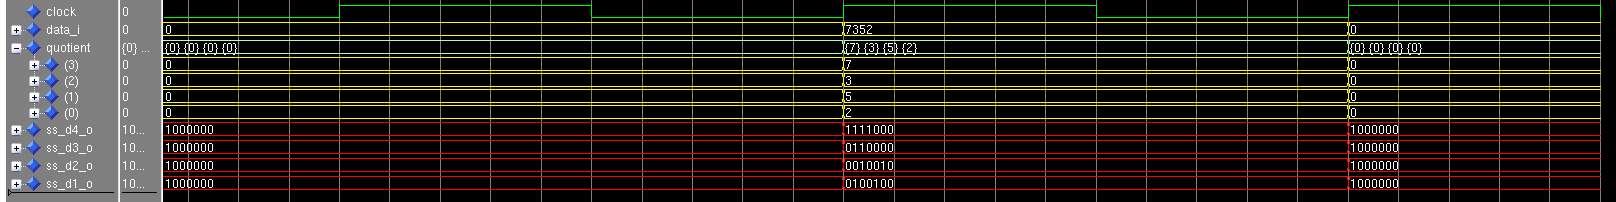
\includegraphics[width=0.98\textwidth]{../Daten/ssd.png}
	\caption{Simulation von ssd.vhd}
	\label{img_ssd}
\end{figure}

Auch dieses Modul wurde natürlich simuliert, zu sehen in Abb. \ref{img_ssd}.
Das Trennen der Dezimalstellen hat offenbar funktioniert.
Es ist zu erkennen, dass die ausgegebenen Signale gerade den erwarteten entsprechen (vergleich mit dem vorherigen Modul).
Bei Änderung der anzuzeigenden Zahlen folgt die Darstellung noch im selben Takt.

\subsection{Modul 5 - \textit{top}}

In diesem letzten Modul werden die anderen vier Module zusammengefasst.
Damit erhält man die gesamte Funktionalität des Filters, der auf Knopfdruck Daten empfängt, den Wiener Filter anwendet, das Maximum bestimmt und dieses dann anzeigt.
Im Folgenden ist der Code des Moduls zu sehen:

\lstinputlisting[firstline = 10]{../Daten/top/top.vhd}

Zuerst sehen wir uns die \textbf{port}s der \textbf{entity} \textit{top} an.
Wir nutzen eine Clock (Zeile $16$), haben einen Button der die Datenaufnahme startet (Zeile $18$), einen Button der das Modul zurücksetzt (Zeile $19$), eine Statusleuchte (Zeile $21$) und die Vier 7-Segment-Anzeigen (Zeilen $23$ bis $26$).
Die Signale in den Zeilen $28$ und $29$ sind für die Kommunikation mit dem PC um die Eingangssignale zu empfangen.

Sehen wir uns nun die \textbf{architecture} an.
Für die Kommunikation zwischen den Modulen müssen wir interne Signale anlegen (Zeilen $37$ bis $40$).
Diese halten die Ergebnisse nach jeder Datenverarbeitung in den Modulen.
Die Module werden eingebunden indem sie instanziiert werden und dann ein mapping angelegt wird.
Zuerst wurde das Modul für das empfangen der Daten vom PC eingebunden (ab Zeile $45$).
Dieses werden wir uns nicht näher anschauen da es für die Funktion des eigentlichen Filters kaum von Bedeutung ist.
Es sei nur darauf hingewiesen, dass in Zeile $66$ die eingehenden Daten auf das Signal data\_raw geschalten werden.
Als nächstes wurde unser Modul \textit{LoHi detect} eingebunden (Zeilen $69$ bis $74$).
Es macht aus dem Knopfdruck das definiertes Startsignal start.
Dann wurde das Modul \textit{filter} eingebunden (Zeilen $76$ bis $84$).
Dort werden die rohen Eingangsdaten wie beschrieben gefiltert und dann in das Signal data\_filtered geschrieben.
Weiter geht es mit dem Modul \textit{Max find} um sequentiell das Maximum der gefilterten Daten zu finden (Zeilen $86$ bis $95$).
Das Maximum der gefilterten Daten wird in dem Signal data\_max gespeichert.
Zuletzt wird das Maximum mit dem Modul \textit{ssd} auf den vier 7-Segment-Anzeigen angezeigt (Zeilen $97$ bis $110$).
Damit ist das Modul top vollständig.

\begin{figure}[ht]
	\centering
    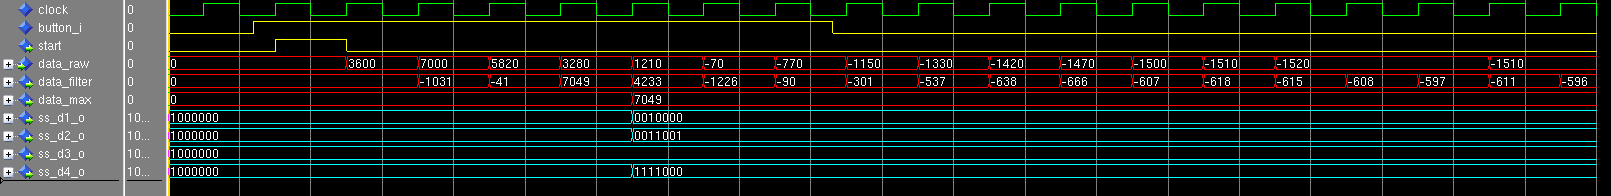
\includegraphics[width=0.98\textwidth]{../Daten/top.png}
	\caption{Simulation von top.vhd}
	\label{img_top}
\end{figure}

Auch dieses letzte Modul wurde zunächst simuliert, zu sehen in Abb. \ref{img_top}.
Man erkennt, dass die Module wie geplant miteinander funktionieren.
Der Knopfdruck wird in ein definiertes Startsignal umgewandelt, zur nächsten steigenden Flanke der Clock werden Daten empfangen.
Nach einem weiteren Zyklus sind die ersten Daten aus dem Filter berechnet.
Negative Zahlen werden beim finden des Maximums ignoriert (bzw. $0$ ist größer als die negativen Werte und wird daher beibehalten).
Das Maximum $7049$ wird bald erkannt und sofort für die 7-Segment-Anzeigen übersetzt.

Damit blieb nur noch das Modul \textit{top} in der Praxis zu testen.
Daher wurde das Modul synthetisiert und dem FPGA aufgespielt.

\begin{figure}[ht]
	\centering
    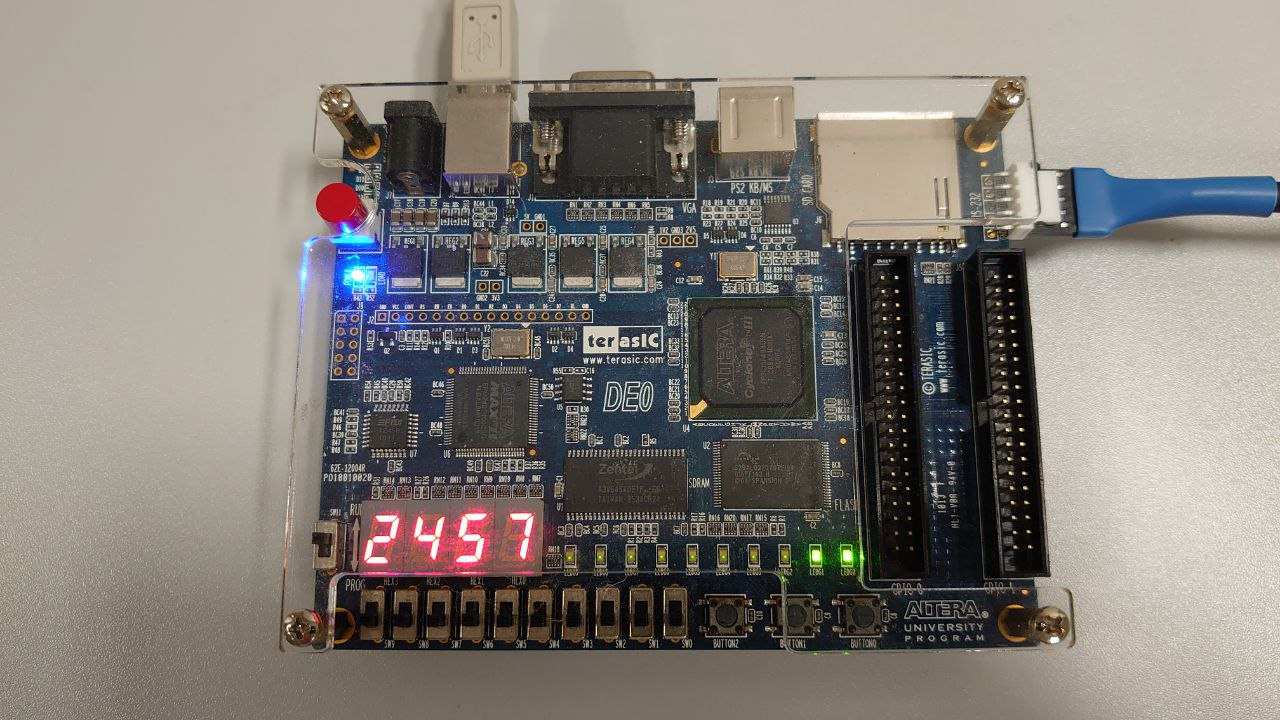
\includegraphics[width=0.98\textwidth]{../Daten/Photo_FPGA_top.png}
	\caption{Photo des FPGA mit aufgespielter, synthetisierter Verknüpfung von top.vhd.}
	\label{photo_top}
\end{figure}

Das Ergebnis kurz nach drücken des Startknopfes ist in Abb. \ref{photo_top} zu sehen.
Hier ist zu erwähnen dass der FPGA sich etwas eigenartig verhalten hat; es war nicht sofort klar welcher Knopf der Start- und welcher der Rücksetzknopf ist.
In jedem Falle sah es für uns so aus als hätte der Test soweit funktioniert.
Ob die $2457$ tatsächlich das richtige Maximum nach anwenden des Filters ist können wir nicht sagen, da wir die eingehenden Daten nicht kennen.



\nocite{*} % alle resourcen auflisten
\printbibliography

% ----- DOKUMENT ENDE -----

\end{document}
